\documentclass[letterpaper, 12 pt]{report}

\usepackage{geometry}
\geometry{a4paper}
\usepackage{siunitx}
\usepackage{graphics}
\usepackage{subcaption}
\usepackage{tikz}
\usepackage{color}
\usepackage{lineno}
\usepackage{hyperref}
\hypersetup{
	colorlinks,
	linktoc=all,
	citecolor=blue,
	filecolor=black,
	linkcolor=black,
	urlcolor=blue
}

\begin{document}
\title{McCAD v1.0 \\ User Manual}
\author{Moataz Harb \\ moataz.harb@kit.edu \\ Karlsruhe Institute of Technology (KIT), Hermann-von-Helmholtz-Platz 1, \\ 76344 Eggenstein-Leopoldshafen, Germany}
\maketitle
\pagestyle{empty}

% -------------------------------------------------------------------------------------
% TABLE OF CONTENTS
% -------------------------------------------------------------------------------------
\tableofcontents
\newpage

% -------------------------------------------------------------------------------------
% INTRODUCTION
% -------------------------------------------------------------------------------------
\section{Introduction}
McCAD is a C++ library for the conversion of CAD solid models to MCNP input syntax, from Boundary Representation "BREP" to Constructive Solid Geometry "CSG".

% -------------------------------------------------------------------------------------
% Installation
% -------------------------------------------------------------------------------------
\section{Installation from Source}
Building of the McCAD library is supported on both Linux and Windows operating systems. The library has three 3rd-party dependencies: CMake, Boost C++ libraries, and Open CASCADE Technology. CMake is the standard build system for McCAD and it comes by default with most Linux distributions as well as Windows OS. Boost C++ libraries consist of header files that are utilized for parallel processing in McCAD. Open CASCADE Technology (OCCT) is used as a geometry engine for geometrical solids manipulation and decomposition. Below are guiding steps for installation on both Linux and Win systems. 
  \subsection{Linux}
    Listed below are the currently supported Linux distributions:
    \begin{itemize}
  	  \item Ubuntu 20.04 LTS
  	  \item Ubuntu 18.04 LTS
    \end{itemize} 
    Testing of installation on other distributions is still underway! thus Ubuntu is recommended as a distribution to install McCAD. Below are general steps to install McCAD code and its dependencies.
    \begin{itemize}
  	  \item \textbf{CMake}
  	  \begin{itemize}
		\item Download cmake-3.23.0.tar.gz from \url{https://cmake.org/download/} then execute the commands below in a terminal.
		\item \$ tar -xzvf cmake-3.23.0.tar.gz
		\item \$ cd cmake-3.23.0
		\item \$ mkdir build
		\item \$ cd build
		\item \$ cmake .. -DCMAKE\_USE\_OPENSSL=OFF -DCMAKE\_INSTALL\_PREFIX=.
		\item \$ make
		\item \$ make install
  	  \end{itemize}
      \item \textbf{Boost C++ liraries}
      \begin{itemize}
    	\item Download boost\_1\_78\_0.tar.gz from \url{https://www.boost.org/users/download/} then execute the commands below in a terminal.
    	\item \$ tar -xvzf boost\_1\_78\_0.tar.gz
    	\item \$ cd boost\_1\_78\_0
    	\item \$ mkdir build
    	\item \$ cd tools/build
    	\item \$ ./bootstrap.sh
    	\item \$ ./b2 install -\--prefix=../../build/
      \end{itemize}
      \item \textbf{Open CASCADE Technology (OCCT)}
      \begin{itemize}
        \item \emph{NOTE}: the instructions on the installation of dependencies can be found on the side menu in \url{https://dev.opencascade.org/doc/occt-7.5.0/overview/html/index.html} by navigating to "Build, Debug and Upgrade $>$ Build 3rd-parties" then following the instructions under "Installation from Official Repositories".
    	\item Download opencascade-7.5.0.tgz from \url{https://dev.opencascade.org/release/previous} then execute the commands below in a terminal.
    	\item \$ tar -xzvf opencascade-7.5.0.tgz
    	\item \$ cd opencascade-7.5.0
    	\item \$ mkdir build
    	\item \$ cd build
    	\item \$ cmake .. -DCMAKE\_BUILD\_TYPE=Release -DBUILD\_LIBRARY\_TYPE=Shared \\ -DCMAKE\_INSTALL\_PREFIX=. -DINSTALL\_TEST\_CASES=TRUE \\ -DINSTALL\_DOC\_Overview=TRUE
    	\item \$ make
    	\item \$ make install
      \end{itemize}
	  \item \textbf{McCAD}
	  \begin{itemize}
		\item \emph{NOTE}: building a shared library is recommended! Should a static library be needed, the user has to insure a compliant build of Open CASCADE Technology by changing the build type; -DBUILD\_LIBRARY\_TYPE=STATIC.
		\item \$ git clone \url{https://github.com/inr-kit/McCAD_Library}
		\item \$ cd McCAD\_Library
		\item \$ mkdir build
		\item \$ cd build
		\item \$ CMake .. -DCMAKE\_INSTALL\_PREFIX=. -DBUILD\_STATIC=OFF \\ -DBOOST\_CUSTOM\_ROOT=$<$PATH to boost\_1\_78\_0$>$ -DOCC\_CUSTOM\_ROOT=$<$PATH to opencascade-7.5.0/build$>$ -DBUILD\_RPATH=ON
		\item \$ make
		\item \$ make install
	  \end{itemize}
    \end{itemize}

  \subsection{Windows}
    Listed below are the currently supported Windows versions:
    \begin{itemize}
  	  \item Windows 10
    \end{itemize} 
    Testing of installation on other versions is still underway! Below are general steps to build McCAD library and its dependencies.
    \begin{itemize}
	  \item \textbf{CMake} (optional)
 	  \begin{itemize}
    	\item \emph{NOTE}: If usage of IDE - such Microsoft Visual Studio (VS) - is intended, then installing CMake can be skipped since most IDE builds CMake by default.
 		\item Download and run the installer cmake-3.23.1-windows-x86\_64.msi from \url{https://cmake.org/download/}.
  	  \end{itemize}
	  \item \textbf{Microsoft Visual Studio} (optional)
	  \begin{itemize}
		\item Download and run the "community" installer from \url{https://visualstudio.microsoft.com/downloads/}.
	  \end{itemize}
      \item \textbf{Boost C++ liraries}
      \begin{itemize}
    	\item Download boost\_1\_78\_0.zip from \url{https://www.boost.org/users/download/}.
    	\item Unzip boost\_1\_78\_0.zip.
    	\item Documentation can be found in index.html in the unzipped folder.
      \end{itemize}
      \item \textbf{Open CASCADE Technology (OCCT)}
	  \begin{itemize}
		\item Download and run the installer opencascade-7.5.0-vc14-64.exe from \url{https://dev.opencascade.org/release/previous}.
	  \end{itemize}
	  \item \textbf{McCAD}
	  \begin{itemize}
		\item Download source code from \url{https://github.com/inr-kit/McCAD_Library} by selecting Code $>$ Download ZIP.
		\item Unzip McCAD\_Library.
		\item Open MSVC and select the McCAD\_Library.
		\item From the "Solution Explorer - Folder Review" double click CMakeSettings.json file. This will open the file in IDE. \item Set a "Configuration name". 
		\item Ensure that "Configuration type" is set to "Release" and "Toolset" is set to msvc\_x64\_x64.
		\item Add -DBUILD\_RPATH=ON -DBUILD\_STATIC\_EXE=ON -DBUILD\_SHARED=OFF -DBOOST\_CUSTOM\_ROOT="$<$PATH to boost\_1\_78\_0$>$" -DOCC\_CUSTOM\_ROOT="$<$PATH to OpenCASCADE-7.5.0-vc14-64\textbackslash opencascade-7.5.0$>$" to "CMake command arguments".
		\item From the top menu select "Build $>$ Build All".
		\item From the top menu select "Build $>$ Install McCAD".
	  \end{itemize}
    \end{itemize}

% -------------------------------------------------------------------------------------
% I/O
% -------------------------------------------------------------------------------------
\section{I/O}
In general, there are three types of information that need to be provided to McCAD: geometry model(s), materials assignment, and running parameters. Below, the input pertinent to the decomposition and conversion will be highlighted. The output from McCAD will depend on the mode of execution, as will be described in the following sections.
  \subsection{General}
	The first input to be provided is the input configuration file, McCADInputConfig.i.  When run via a command line \emph{without arguments}, McCAD will generate a template configuration file, figure (\ref{fig:config}), with the default values of the run parameters. In both run modes, decomposition and conversion, McCAD input parameters are needed. The run parameters are assigned values by default and can be modified by the user. Below is a description of the general input parameters.
	\begin{itemize}
		\item \textbf{debugLevel}: the level at which run/debug info is diplayed on the screen. \emph{Default} is 0.
		\item \textbf{units}: The units used in the CAD model. \emph{Default} is cm.
		\item \textbf{inputFileName}: the input STEP file(s) name(s). \emph{Default} is input.stp.
	\end{itemize}

	\begin{figure}
		\centering
		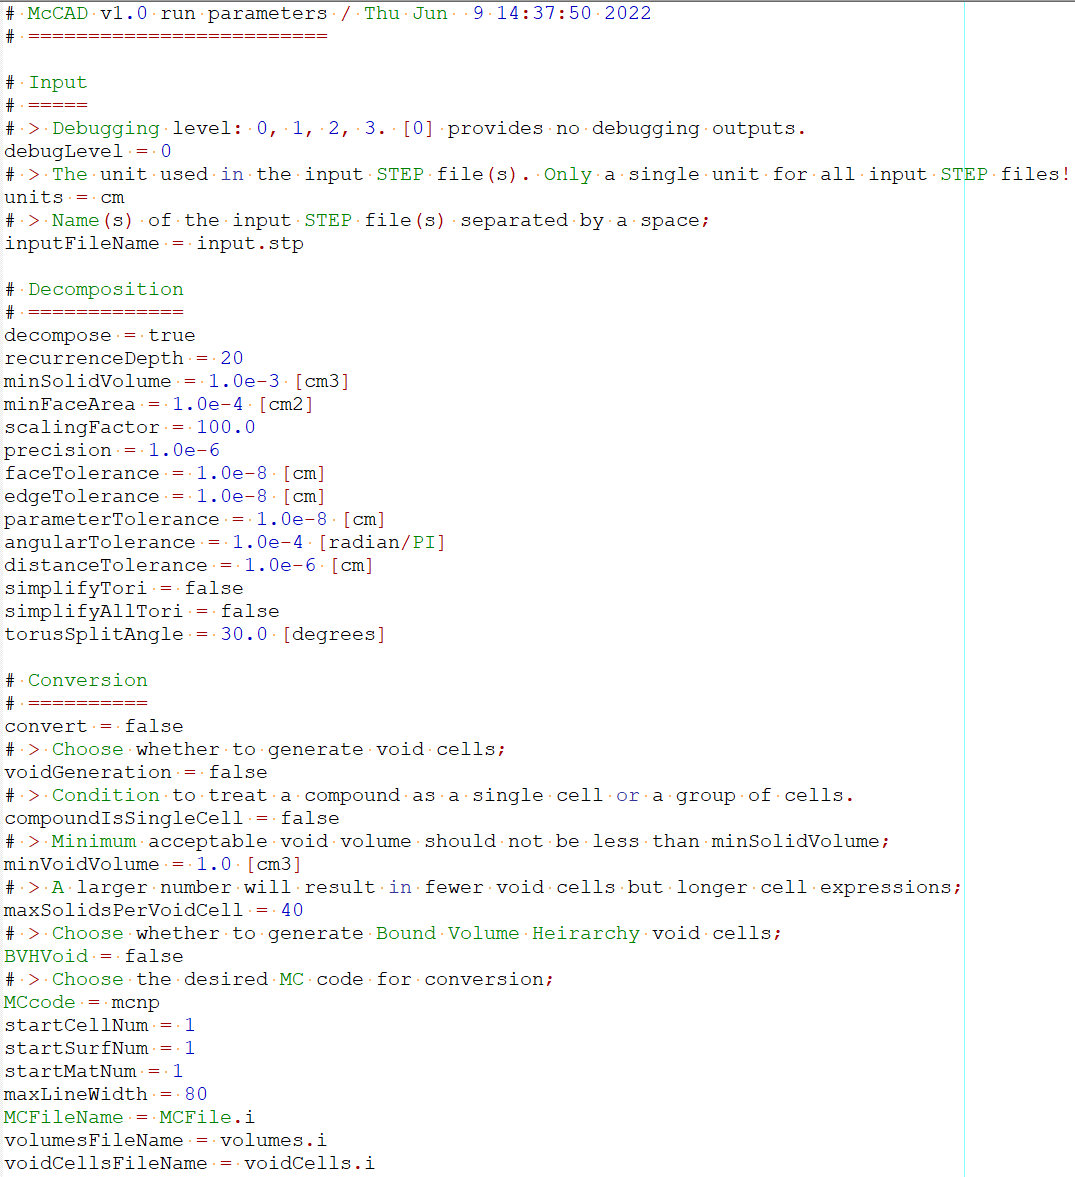
\includegraphics[scale=0.6]{figures/configFile.png}
		\caption{McCAD Input Configuration File}
		\label{fig:config}
	\end{figure}

  \subsection{Decomposition}
    Currently McCAD supports input files in the STEP format (protocol 214). McCAD accepts both single and multiple input STEP files. After successfully running McCAD decomposition two STEP output files will be written to disk. The first will contain the decomposed input solids and the second will contain the rejected/failed input solids. If the latter is absent, this means no input solids were rejected and no solids failed to be decomposed. \\
    \\
    Before running McCAD in the decomposition mode, the user is advised to review the input parameters on the decomposition section on the input configuration file, figure (\ref{fig:config}). Below is a description of the decomposition input parameters.
	\begin{itemize}
	  \item \textbf{decompose}: a logical condition for running decomposition on the input file(s). \emph{Default} is true.
	  \item \textbf{recurrenceDepth}: defines the level of decomposition performed recursively on input solids. This input specifies the maximum number of recursive application of decomposition on the subsolids. The larger the number, the less the failed solids with a lot of detailes in the geometry. \emph{Default} is 20.
	  \item \textbf{minSolidVolume}: this input is used to control the recursive splitting of the solids along with the reciurrenceDepth. It is also used to filter the input solids by rejecting smaller solids than the specified value. \emph{Default} is 1.0e-3 cm\textsuperscript{3}.
	  \item \textbf{minFaceArea}: used to filter the input solids by rejecting solids with faces smaller in area than the specified value. \emph{Default} is 1.0e-4 cm\textsuperscript{2}.
	  \item \textbf{scalingFactor}: controls the size of generated mesh on solids faces. This parameter mainly affects the collision detection of surfaces. More details can be found in section \ref{sec:theory}. \emph{Default} is 100.0.
	  \item \textbf{precision}: used to judge the equality of numerical values. \emph{Default} is 1.0e-6.
	  \item \textbf{faceTolerance}: More details can be found in section \ref{sec:theory}. \emph{Default} is 1.0e-8 cm.
	  \item \textbf{edgeTolerance}: More details can be found in section \ref{sec:theory}. \emph{Default} is 1.0e-8 cm.
	  \item \textbf{parameterTolerance}: More details can be found in section \ref{sec:theory}. \emph{Default} is 1.0e-8 cm.
	  \item \textbf{angularTolerance}: More details can be found in section \ref{sec:theory}. \emph{Default} is 1.0e-4 radian/PI.
	  \item \textbf{distanceTolerance}: More details can be found in section \ref{sec:theory}. \emph{Default} is 1.0e-6 cm.
	  \item \textbf{simplifyTori}: a logical condition on whether or not simplify toroidal solids as a collection of smaller cylindrical segments. If true, only off axis tori will be simplified. \emph{Default} is false.
	  \item \textbf{simplifyAllTori}: a logical condition on whether or not simplify all toroidal solids as a collection of smaller cylindrical segments. If true, all toroidal solids, disregarding its axis, will be simplified. \emph{Default} is false.
	  \item \textbf{torusSplitAngle}: the angle between the top and bottom bases of a cylindrical segment. \emph{Default} is 30.0 degrees.
    \end{itemize}

  \subsection{Conversion}
    McCAD conversion will result in three textual output files. The first contains the generated Monte Carlo, MCNP is only support for now, input file. The second contains a mapping of cell ID, volume, and solid name. The third file contains a mapping of void cell IDs to material cell IDs. More details on the format of the three files can be found in section \ref{sec:example}. \\
    \\
    Material assignment is currently deduced from the name of the STEP files. The user is advised to split the CAD model into several by material. The name of the input STEP files takes the format $<$material name$>_<$density in exponential format: -0.0E0$>_<$.stp. The material name and density are then extracted from the file name and assigned to the solids it contains. For MCNP, the sign of the density implies whether mass or atomic densities is used. In case of absence of the density value, void is assumed. It is important to note that the underscore only separates the material name from density. Any extra underscores will result in an error. \\
    \\
    Before running McCAD in the conversion mode, the user is advised to review the input parameters on the conversion section on the input configuration file, figure (\ref{fig:config}). Below is a description of the decomposition input parameters.
	\begin{itemize}
	  \item \textbf{convert}: a logical condition for running conversion on the input file(s). \emph{Default} is false.
	  \item \textbf{voidGeneration}: a logical condition for void generation. If false, only a single void cell is created outside which is a graveyard. \emph{Default} is false.
	  \item \textbf{compoundIsSingleCell}: controls whether to define the subsolids of the decomposid input solid into separate cells or unify it through the union operator into a single cell. If true, all subsolids are joined  through a union operator and a single cell is written to the MC input file. This is not recommended for complex solids since it slows down the transport due to the many surface crossing checks. \emph{Default} is false.
	  \item \textbf{minVoidVolume}: controls the desirable minimum void cell volume. \emph{Default} is 1.0 cm\textsuperscript{3}.
	  \item \textbf{maxSolidsPerVoidCell}: this input will control the number of generated void cells. A smaller number will result in a larger number of void cells each with simpler expression on the MC file. \emph{Default} is 40.
	  \item \textbf{BVHVoid}: a logical condition for generating a bound volume hierarchy void cells. This feature is still undergoing testing and not currently recommended to be used. \emph{Default} is false.
	  \item \textbf{MCcode}: specifies the targeted MC code to generate the input file in a compliant format. Currently only MCNP is supported. \emph{Default} is mcnp.
	  \item \textbf{startCellNum}: the desired starting cell number. \emph{Default} is 1.
	  \item \textbf{startSurfNum}: the desired starting surface number. \emph{Default} is 1.
	  \item \textbf{startMatNum}: the desired starting material number. \emph{Default} is 1.
	  \item \textbf{maxLineWidth}: maximum length of lines on the MC file. \emph{Default} is 80.
	  \item \textbf{MCFileName}: the desired name for the MC file. \emph{Default} is MCFile.i.
	  \item \textbf{volumesFileName}: the desired name for the cell ID-volumes-name mapping file. \emph{Default} is volumes.i.
	  \item \textbf{voidCellsFileName}: the desired name of the void to material cells mapping file. \emph{Default} is voidCells.i.
    \end{itemize}

\section{Running McCAD}
There are two ways to run McCAD, via a command line or the SpaceClaim plugin. McCAD can be run from a command line either in a Linux terminal or a Windows command prompt.

  \subsection{Command Line}
    On a linux termial of Windows command prompt McCAD can be run by typing in the path to the executable followed by the desired argument. A good practice is to add the path to the McCAD executable to the PATH environment variable then simply call McCAD with the acceptable desired command line arguments. The arguments could be displayed on the screen by running "McCAD help". The acceptable McCAD arguments are listed below.
    \begin{itemize}
    	\item \textbf{[]}: running McCAD without arguments will result in writing McCAD template input configuration file, McCADInputConfig.i.
    	\item \textbf{[help]}: lists all the acceptable arguments.
    	\item \textbf{[read]}: test loading the solids from the input STEP file(s). This is used to test if the OCCT reader will fail to load any STEP file(s).
    	\item \textbf{[run]}: executes McCAD according to the selected running mode: decomposition, conversion, or both. 
    \end{itemize}

  \subsection{SpaceClaim Plugin}
    The python script located in SpaceClaim\_interface can be loaded into SpaceClaim and used directly to call McCAD to perform decomposition on selected solid(s).  The script can be loaded in SPaceClaim by selecting "File $>$ New $>$ Script". Select the desired solid(s) to decompose and on the "Script Editor" select "Run Script", the green arrow.

% -------------------------------------------------------------------------------------
% Notes on Usage
% -------------------------------------------------------------------------------------
\section{Example} \label{sec:example}
General notes on how to use McCAD. Coming soon ...
  \subsection{Decomposition}
  \subsection{Conversion}
  \begin{itemize}
	\item Coordinates
  \end{itemize}


% -------------------------------------------------------------------------------------
% Knows Issues
% -------------------------------------------------------------------------------------
\section{Known Issues}
A list of known issues and how to manually fix it in solid models. Coming soon ...
\subsection{Decomposition}
\begin{itemize}
	\item simplifying of tori
	\item hollow solids
	\item splitting of cylinders and tori
\end{itemize}
\subsection{Conversion}


% -------------------------------------------------------------------------------------
% Theory of McCAD Conversion
% -------------------------------------------------------------------------------------
\section{Theory of McCAD Conversion} \label{sec:theory}
Comperhensive details on the inner workings of McCAD classes for developers. Coming soon ...
\subsection{Decomposition}
\subsection{Conversion}
\newpage
% -------------------------------------------------------------------------------------
% REFERENCES
% -------------------------------------------------------------------------------------
%\bibliography{}

% -------------------------------------------------------------------------------------
% END DOCUMENT
% -------------------------------------------------------------------------------------
\end{document}